\documentclass[conference]{IEEEtran}
\IEEEoverridecommandlockouts
\usepackage{cite}
\usepackage{amsmath,amssymb,amsfonts}
\usepackage{algorithmic}
\usepackage{graphicx}
\graphicspath{{img/}}
\usepackage{textcomp}
\usepackage[table]{xcolor}
\usepackage{verbatim}
\usepackage{tabularx}
\usepackage{listings}
\usepackage{xcolor}
\usepackage{hyperref}
\hypersetup{
    colorlinks=true,
    linkcolor=blue,
    filecolor=magenta,      
    urlcolor=cyan,
}
\definecolor{codegreen}{rgb}{0,0.6,0}
\definecolor{codegray}{rgb}{0.5,0.5,0.5}
\definecolor{codepurple}{rgb}{0.58,0,0.82}
\definecolor{backcolour}{rgb}{0.95,0.95,0.92}
\lstdefinestyle{mystyle}{
    backgroundcolor=\color{backcolour},   
    commentstyle=\color{codegreen},
    keywordstyle=\color{magenta},
    numberstyle=\tiny\color{codegray},
    stringstyle=\color{codepurple},
    basicstyle=\ttfamily\footnotesize,
    breakatwhitespace=false,         
    breaklines=true,                 
    captionpos=b,                    
    keepspaces=true,                 
    numbers=left,                    
    numbersep=5pt,                  
    showspaces=false,                
    showstringspaces=false,
    showtabs=false,                  
    tabsize=2
}
\lstset{style=mystyle}
\def\BibTeX{{\rm B\kern-.05em{\sc i\kern-.025em b}\kern-.08em
    T\kern-.1667em\lower.7ex\hbox{E}\kern-.125emX}}
    
    
\begin{document}


\title{Cosmic\\A Software Simulated 8-Bit Computer Architecture}
\author{\IEEEauthorblockN{Clay Buxton}
\IEEEauthorblockA{\textit{Computer Engineering, Computer Science} \\
\textit{Elizabethtown College}\\
Elizabethtown, PA \\
buxtonc@etown.edu}
\and
\IEEEauthorblockN{Kevin Carman}
\IEEEauthorblockA{\textit{Computer Engineering, Computer Science} \\
\textit{Elizabethtown College}\\
Elizabethtown, PA \\
carmank@etown.edu}
}
\maketitle


\begin{abstract}
The Cosmic processor, graphical user interface (GUI), and assembler aim to educate students with little or no knowledge of computer architecture or assembly language. Derived from 8-bit processors of the 1980’s, Cosmic was built with simplicity and modularity in mind. The simplicity is in the fundamentally basic and well-documented instruction set, while the modularity stems from the design of the system. The system was designed in a way that anyone could write their own simulation environment, graphics stack, peripherals, drivers, and more to use the Cosmic processor at its core. Written in C++ and Python with minimal dependencies, Cosmic is lightweight and portable, which makes it perfect for running on almost any system, including running headless on systems with low graphical power. While no experimentation on its educational properties has currently been conducted, Cosmic is ready with informative labs for students to engage with. Modern, complex assembly languages will no longer be a starting point for novice programmers.
\end{abstract}

\begin{IEEEkeywords}
retro-computing, simulation, emulation, microprocessor, 8-bit architecture.
\end{IEEEkeywords}


\section{Introduction}
One of the biggest problems Computer Science students face today is low-level programming. Between archaic languages, expensive hardware, and incomplete or scattered documentation, low-level programming is not only intimidating, but also difficult to learn. Cosmic seeks to remedy all of this with a modern, well documented, and simple language alongside an easy to use interface, and support for hardware that you already own. Along with three labs we developed Cosmic, is a easy, free, and open source way to either learn low level programming, or create your own virtual computer. 


\section{Background}
The largest source of background information is in the machines that Cosmic is designed to resemble. The two primary reference devices are the Apple II and the TRS-80 containing the MOS 6502 and the Zilog Z80, respectively.

There are a few other projects out there that are similar to what we did. Emulators of similar devices were helpful for design inspiration. Unlike emulators, we do not have the same design constraints, which added a sense of freedom when creating the system. Outside of emulators, there are a few projects where developers have created self-defined simulated platforms. One such project is an 8-bit Assembler and Simulator written by Marco "Schweigi" Schweighauser\cite{b1}. Another project that influenced the creation of Cosmic is David Murray's Commander X16 project\cite{b2}. Unlike the Assembler-Simulator, this is a "home-brew" physical computer made using off-the-shelf parts. This project uses the 6502 and other components to create a retro-feeling machine with more modern parts. 

Our project is a little big different. We've greatly expanded on the simple processor that was in the "Assembler and Simulator" to a full blown instruction set, support for I/O and a much more fleshed out interface. Our processor is also completeley new, and runs all in software so it's a bit more flexible and a lot cheaper than the still in development Commander X16. 

Luckily, devices of the time have been very well documented in the past 40 years. This documentation made reverse-engineering the systems and processors simple and allowed us to figure out how engineers of yesterday solved problems that we encountered while designing our system. 


\section{Design Constraints}
At the core of the system, we wanted to follow three rules. First, keep it simple. Cosmic uses a RISC-like instruction set, each instruction has one simple task to do. All of the instructions are an opcode and operand excluding MOV which takes 2 operands for ease of use. Cosmic is 100\% memory mapped so nothing is hidden from the user and everything is adjustable. Changes in I/O, Graphics, and the like are always view-able and editable. The second rule was to follow proper software engineering methodologies. We wanted Cosmic to be an example of how to write clean code, use resources available to us, and test everything. We followed this very well with our testing, automated builds, and project structure. The final rule was that it was open source and modular, so anyone could see how Cosmic works under the hood and even add their own instructions, peripherals, and additions to the GUI. We made it very easy for anyone to add anything they want to the processor.


\section{Timeline}

\subsection{Fall Semester}
Fall semester was the beginning of Cosmic, so much of the semester involved planning and design. Everything from picking the instructions we wanted to implement, to designing the GUI, to planning the underlying system (memory, graphics, etc.) was done during this phase.

By the end of the fall semester, we had the Cosmic processor mostly developed and tested, which was the most important task during this time. Alongside that, the GUI was was developed to a significant working extent and we just scratched the surface in regards to writing the assembler.


\subsection{Spring Semester}
Spring semester kicked off with a heavy focus on finishing development of the assembler and then transitioned to implementing a video output screen and a plethora of GUI improvements. As the semester progressed, focus on developing Cosmic shifted to begin preparing for SCAD. This included tasks such as recording a video presentation, designing a poster, and writing three labs to showcase our project and its educational value. Luckily, among the chaos, we still had time to implement interfacing hardware with Cosmic such as keyboard inputs and GPIO pins on a Raspberry Pi. In the end, all of our deliverables were met.


\section{Budget}
At first, we thought since our entire project is in software, that nothing would need to be bought. As development continued, we decided to purchase two 4GB Raspberry Pis to experiment interfacing Cosmic with real-world hardware. For just under \$90 each, these Raspberry Pis greatly outclassed the under-powered ones that were available for use in the Elizabethtown Computer Engineering lab. Two of them were purchased so that each one of us could experiment with them in our own way on our own time without having to worry about conflicting with each other and the classes that use the already available.


\section{Social, Ethical, and Environmental Impacts}

\subsection{Social Impacts}
Our project doesn't have any direct social impacts. It's a project that many people will find interesting and that could be useful in an educational environments.

\subsection{Ethical Impacts}
The biggest ethical factor of our project is about the code itself. We decided to keep the project 100\% open source. We think this is important for a project like this to allow others to learn from our design. All of the libraries included are also all open source.

\subsection{Environmental Impacts}
Our project will have no impact on the environment, as it will be written entirely in software. Hardware that is interfaced with Cosmic such as Raspberry Pis will be completely reusable afterwards.


\section{Design}
\subsection{Bitness}
The "bitness" of a chip is traditionally the size of the data bus. An 8-bit chip can address 8 bits of data at one time, a 16-bit chip can address 16 bits of data etc.

Our design choice was between an 8-bit design and a 16-bit design. 32-bit and 64-bit designs were not considered as they did not exist during the time that the chips that Cosmic is similar to were made.\\

\resizebox{\columnwidth}{!}{%
 \begin{tabular}{||c|c|c|c|c||}
 \hline
 Factors & Practical Use & Implementation & Appropriate Design & \cellcolor{blue!40}Total\\ [0.5ex] 
 \hline\hline
 Weights & 3 & 2 & 2& \\ 
 \hline
 8-bit & 5 &  8&  9 & \cellcolor{blue!25}49\\
 \hline
 16-bit  &  8 & 5 &  5 & \cellcolor{blue!25}44\\
 \hline
\end{tabular}
}\\

An 8-bit chip was chosen mainly due to it being more relevant to the class of chips Cosmic is made to fit in with, those of the early 80's and late 70's. A 16-bit chip would have been slightly more work to implement, but would have been much more useful to write for.

\subsection{Registers vs. Zero Page vs In-Memory Registers}

Chips of the time generally had registers in 3 formats. There were many registers separated from memory like in the Z80. Few registers and then an easily accessible portion of memory like in the 6502. Or on chips with on-board memory, the registers would take up the first few bytes of memory.

Each of these has it's pros and cons, but all configurations were designed with two things in mind, speed and utility. On a physical chip, retrieving data from a register is significantly faster than a location in memory, but you only had 8 bytes. Getting something from zero page memory on the 6502 was faster than getting something from another place in memory, but slower than a register, but you had 256 bytes.\\

\resizebox{\columnwidth}{!}{%
 \begin{tabular}{||c|c|c|c|c||}
 \hline
 Factors & Practical Use & Implementation & Appropriate Design & \cellcolor{blue!40}Total\\ [0.5ex] 
 \hline\hline
 Weights & 3 & 2 & 2& \\ 
 \hline
 Many Registers & 9 &  8&  10 & \cellcolor{blue!25}63\\
 \hline
 Zero Page  &  5 & 5 &  10 & \cellcolor{blue!25}45\\
 \hline
 Onboard Memory &  6 & 10 &  7& \cellcolor{blue!25}52\\

 \hline 
\end{tabular}
}\\

Registers, similar to the Z80 made the most sense in our case. Since there is no speed difference between accessing zero page and accessing any other position in memory in our design, zero page addressing would be a waste of time to implement. On-board memory would have been very easy to develop, but was generally found on microcontrollers rather than microprocessors, and would have held no real speed boost either.

\subsection{16-Bit Register Mode}
16-bit register mode is when two of the 8-bit registers can be used together to act as a 16-bit register. This can also be done for certain instructions as well.\\

\resizebox{\columnwidth}{!}{%
 \begin{tabular}{||c|c|c|c|c||}
 \hline
 Factors & Practical Use & Implementation & Appropriate Design & \cellcolor{blue!40}Total\\ [0.5ex] 
 \hline\hline
 Weights & 3 & 2 & 2& \\ 
 \hline
 No 16 Bit mode & 4 &  8&  10 & \cellcolor{blue!25}48\\
 \hline
 16 Bit mode &  10 & 6 &  10 & \cellcolor{blue!25}62\\
 \hline
\end{tabular}
}\\

Overall, a 16-bit mode was a good decision. This allows for a lot more usability, and still fits in with chips of the time since the Z80 also had 16-bit mode instructions. This did add a bit of work, significantly increasing our instruction count,  but was worth it overall.

\subsection{Signed vs. Unsigned Data}

During the design we were unsure how to use signed and unsigned numbers. In the Z80 and 6502 there is no distinction between the two in position of memory since the arithmetic functions do binary math. The programmer must keep track of if the number is signed or unsigned and flags are used in math to signify certain cases.\\

\resizebox{\columnwidth}{!}{%
 \begin{tabular}{||c|c|c|c|c||}
 \hline
 Factors & Practical Use & Implementation & Appropriate Design & \cellcolor{blue!40}Total\\ [0.5ex] 
 \hline\hline
 Weights & 3 & 2 & 2& \\ 
 \hline
 Specifically Signed Data & 8 &  4 &  3 & \cellcolor{blue!25}38\\
 \hline
 Overflow and Carry flags &  5 & 8 &  7 & \cellcolor{blue!25}45\\
 \hline
\end{tabular}
}\\

While having specifically signed functions and locations would have been helpful, it would have been a lot to implement and not really consistent with how processors work. Instead we focused on having flags when using arithmetic functions show if things would be negative and when it would overflow.

\subsection{Op-code Selection}

The op-code selection is the control logic of a simulated chip. It takes an op-code in from memory and has to resolve it to a instruction to execute. This can be done in a few ways. One way is using a large switch statement to branch to the proper instruction function. This can be large and cumbersome, but is also very simple. Another way is to use function pointers and then store them in a way in which they can be easily called. We could also create a struct to hold the function pointer and then other things relevant to the instruction like size, mnemonic, and addressing mode.\\

\resizebox{\columnwidth}{!}{%
 \begin{tabular}{||c|c|c|c|c||}
 \hline
 Factors & Practical Use & Implementation & Appropriate Design & \cellcolor{blue!40}Total\\ [0.5ex] 
 \hline\hline
 Weights & 3 & 2 & 2& \\ 
 \hline
 Switch Statement & 3 & 10& n/a& \cellcolor{blue!25}29\\
 \hline
 Function Pointers &  7& 7&  n/a& \cellcolor{blue!25}35\\
 \hline
 Function Pointers w/ Data &  9 & 7 &  n/a & \cellcolor{blue!25}41\\
 \hline
\end{tabular}
}\\

A switch statement is very large and cumbersome and also is a very crude way to select op-codes. We decided using an array of structs containing the function pointers, and additional data about the function way the best way to go. While it was tricky to implement, it works very well, is much faster than a switch statement, and also contains a lot of data about each of the functions. The instructions are put into an array at the position that their op-code is. For instance the NOP instruction is op-code 0x00, so it was put into the first element of the array so when InstructionSet[0] is called, it will return the struct which contains the function pointer for the NOP instruction

\subsection{Addressing functions}

When writing the functions for the op-codes, we were unsure on how to implement the addressing modes. They could either be done as separate functions or each instruction could be implemented separately with its addressing mode.\\

\resizebox{\columnwidth}{!}{%
 \begin{tabular}{||c|c|c|c|c||}
 \hline
 Factors & Practical Use & Implementation & Appropriate Design & \cellcolor{blue!40}Total\\ [0.5ex] 
 \hline\hline
 Weights & 3 & 2 & 2& \\ 
 \hline
 Individual Functions & 3 &  7&  n/a & \cellcolor{blue!25}23\\
 \hline
 Addressing Functions &  7 & 6 &  n/a & \cellcolor{blue!25}33\\
 \hline
\end{tabular}
}\\

Implementing each function with each addressing mode was very cumbersome as it increased the number of instruction functions significantly. Although 2 different functions have to be written for each function due to the way our addressing works, it reduced the total number of functions and made writing the remaining functions very easy. 

\subsection{GUI back-end}

The GUI back-end for the simulation environment was the smallest design decision to make. The main decision had to be made between immediate or a retained mode GUI. Qt4 ,a retained mode GUI and ImGUI, a immediate mode GUI were both libraries we were familiar with and could easily implement. \\
The GUI back-end for the simulation environment was the least significant design decision to make. The main decision had to be made between immediate or a retained mode GUI. Qt4 ,a retained mode GUI, and ImGui, an immediate mode GUI, were both libraries we were familiar with and could easily implement. \\

\resizebox{\columnwidth}{!}{%
 \begin{tabular}{||c|c|c|c|c||}
 \hline
 Factors & Practical Use & Implementation & Appropriate Design & \cellcolor{blue!40}Total\\ [0.5ex] 
 \hline\hline
 Weights & 3 & 2 & 2& \\ 
 \hline
 ImGui & 8 &  5&  n/a & \cellcolor{blue!25}34\\
 \hline
 Qt4 &  6 & 5 &  n/a & \cellcolor{blue!25}23\\
 \hline
\end{tabular}
}\\

We chose immediate mode due to how much would be changing on screen at a time, and since the elements in the GUI would not be super intensive, and ImGui is much easier to implement and works cross platform with few external dependencies.




\subsection{Supported Systems}

Targeting all operating systems can be difficult since they all require different dependencies and have different ways to build the software. macOS and Linux work similarly enough for our purposes and very few changes have to be made to the build process between macOS and Linux. Windows however requires a different process and generally requires tools installed that most people will not unless they are writing in C/C++ without Microsoft tools. \\

\resizebox{\columnwidth}{!}{%
 \begin{tabular}{||c|c|c|c|c||}
 \hline
 Factors & Practical Use & Implementation & Appropriate Design & \cellcolor{blue!40}Total\\ [0.5ex] 
 \hline\hline
 Weights & 3 & 2 & 2& \\ 
 \hline
 Windows, macOS, \& Linux & 8 &  5 &  n/a & \cellcolor{blue!25}34\\
 \hline
 macOS \& Linux &  6 & 7 &  n/a & \cellcolor{blue!25}32\\
 \hline
\end{tabular}
}\\

\section{Testing Methodologies}
Cosmic was designed to be modular for developers to be able to create their own parts of the system. A byproduct of this also made Cosmic incredibly easy to test. We made a significant effort to automate as much of the testing as possible to verify that the builds we produce are stable on any platform.

While testing Cosmic, we use three primary ways of testing the system, assembler, and any other correlated code.

\subsection{Unit Testing}
Unit testing is a great way to make sure that parts are working exactly as we expect them to as things get updated and features get added. Currently, the only portion of the project that is unit tested is the Cosmic Processor itself. As of the writing of this document, we have 565 assertions over 54 different test cases that are all passing. These tests check each instruction in a variety of different ways to make sure that they are working as intended. Not only does this provide a great way to make sure the processor is working correctly, but while writing these tests, we found numerous bugs throughout the processor. Listing \ref{test1} shows an example of one of the many test cases for the SHLX Instruction. 
\begin{lstlisting}[language={C++}, caption={A unit test for the SHLX instruction.}, label = {test1}]
/* 0x4C-0x4F */
TEST_CASE("shlx", "[opcodes]"){
    cosproc proc = cosproc(MemoryRead, MemoryWrite);
    //Imm
    /*
    0000: 4C 00 01 ...
    */
    reset(&proc);
    memory[0x00] = 0x4C;
    memory[0x02] = 0x01;
    proc.r[0] = 0x44;
    proc.r[1] = 0x22;
    proc.cycle();
    REQUIRE(proc.r[0] == 0x88);
    REQUIRE(proc.r[1] == 0x44);
}
\end{lstlisting}

We set up the processor and memory to properly execute the test case we are trying to replicate. The processor then executes the instructions and the memory, registers, or flags are checked depending on the purpose of the test. For the processor, we used Catch2\cite{b3} to write our unit testing, a multi-paradigm test framework for C++. In the future, the unit tests will be written for the assembler using the pytest\cite{b4} framework.

\subsection{Manual Testing}
Since the majority of the system is not thoroughly tested or is difficult to test (ex. GUI), manual testing is done to ensure that everything is working well and doesn't break. This constitutes us going in and trying to do everything from using the project normally, to breaking the GUI, to running edge cases. While this helps us discover bugs, it also encourages us to think of ways to improve the GUI and the overall usability of our project. While our unit tests focus on individual instructions or functions, our manual tests ensure that the entire system as a whole is working accordingly.

\subsection{Automated Testing}
Using Travis CI\cite{b5}, every time we push an update or change to our GitHub repository, it kicks off several separate builds of the Cosmic system. Cosmic gets compiled and tested on five different environments; x86, ARM, Linux, Windows, and macOS. These builds compile in a clean environment to ensure that the system can compile and run correctly across each platform, not just the systems we are using to design it. The builds start by cloning the repository, then downloading the necessary packages, then finally compiling and running our unit tests. After the builds are complete, we get notified if something causes them to fail so that we know what to fix.

\subsection{Testing Results}
Using the results of our manual and automated testing, we track bugs and other issues using GitHub. Whenever a bug, undesired behavior, or improvement needs to be made, an issue is opened on GitHub and tracked in our Project tracker. The bug is then cataloged, assigned, and worked on. Once it's verified that the bug is squashed, the issue is then closed.


\section{Results}
Three introductory labs were created to teach how to write assembly and utilize Cosmic in an educational environment as well as show off some of the features of Cosmic. The labs are generated from a compact and clean LaTeX template, and are easily editable and reusable. They include information such as the lab objective, a prelab section that asks the students to familiarize themselves with specific instructions or other key aspects of Cosmic beforehand, a during lab section that lays out the problem the students must solve, a grading section that breaks down exactly what is required of the student for the lab, and a helpful links section that directs to Cosmic documentation and other helpful places.

\subsection{Basic Operations}
The first lab asks the student to calculate and the nth Fibonacci number. Since our processor, is only 8 bits, the following constraint is applied: 1 $\leq$ n $\leq$ 13. This lab teaches the basics of Cosmic, such as using instructions, variables, and loops in the assembler to carry out simple tasks. A sample solution is shown in Listing \ref{lab1}.

\begin{lstlisting}[caption={Cosmic assembly to find the nth Fibonacci number.}, label = {lab1}]
byte fib = 6
;The Fibonacci number we wish to calculate
byte counter = 2
byte first = 0
byte second = 1
;Initialize the first two numbers in the sequence to be 1
byte final = 0
JMP #08
end:
    MOV R0 final
    HCF
    ;End of program
MOV #1 R0
CMP fib
JZS #end
;Check to see if fib is 1
calculate:
    MOV first R0
    ADD second
    MOV second first
    MOV R0 second
    MOV fib R0
    CMP counter
    MOV second R0
    ;Needed since we store R0 in final
    JZS #end
    INC counter
    JMP #11
\end{lstlisting}

Since we are calculating the nth Fibonacci number, we stored our n, in this case 6, as fib. A Fibonacci number is calculated by adding together the previous two numbers in the sequence, so we stored the first and second numbers of the sequence accordingly. We defined a counter variable to keep track of which Fibonacci number we are on, and we initialize it to two because if we want the first number in the sequence, we can just return 1 without any calculations. Lastly, we defined a final variable to store our answer in. We then defined an end loop, which is only called after we have generated our answer, to store our final answer in. The MOV, CMP, and JZS instructions following the end of the end loop act as an if statement to check is fib is equal to 1. If it is not, then we head into the calculate loop. This loop moves our first variable into the accumulator and adds the second to it. Then it moves the second variable to the first, and the accumulator to the second. It then checks to see if we have calculated the nth Fibonacci number or not. If we need to continue calculating, the counter is incremented and JMP is called to bring us back to the start of the calculate loop. If the answer has been found, the end loop is called and the program ends after it executes. After the program ends, 8, the 6th Fibonacci number, should be stored in the final variable.

After a program like the one found in Listing \ref{lab1} is written, it is as simple as clicking Assemble in the Cosmic editor to assemble the code into machine code and load it into the memory editor. All the user has to do afterwards is simply click Run to start executing the program.

\subsection{Basic Graphics}
The second lab asks the student to write a program to output a gradient to the Cosmic video screen. Since Cosmic's video output works by reading the video memory for brightness values for each pixel, ranging from 0x00 to 0xFF, the student must loop through the video memory and store either decreasing or increasing values of brightness for the pixels. This lab again reinforces the basics of Cosmic and introduces the usage of the video output. A sample solution is shown in Listing \ref{lab2}.

\begin{lstlisting}[caption={Cosmic assembly to output a gradient to the video screen.}, label = {lab2}]
byte brightness = FE
;Start at full brightness -1 so that the program terminates correctly.
word start = 8000
;Starting pixel
MOVX #BFFF R0
;Store the end location of the video memory.
loop:
	MOV brightness @start
	;Set the brightness of this pixel
	DEC brightness
    DEC brightness
    ;Decrement the brightness by two because the video out is 64x64
	INCX start
	CMPX start
	JNZ #loop
	;Repeat until the brightness reaches 0
HCF
;End of program
\end{lstlisting}

Since Cosmic's video screen is 64x64, we define our initial brightness to be 0xFE. We also define a word, 16 bits instead of 8 bits, starting location for the beginning of the video memory. We then MOV the end location of the video memory to the 16-bit accumulator as a reference. Next, we defined a loop to MOV the current brightness value to the current pixel in video memory. We then decrement the brightness variable twice, since each line of the video screen is only 64 pixels long, and increment our position in video memory. Lastly, we compare our position in video memory to the accumulator, since we stored the end location there, to determine if we should continue drawing or end the program. The outcome is a smooth gradient as can be seen in Figure \ref{fig:gradient}.

\begin{figure}[h!]
	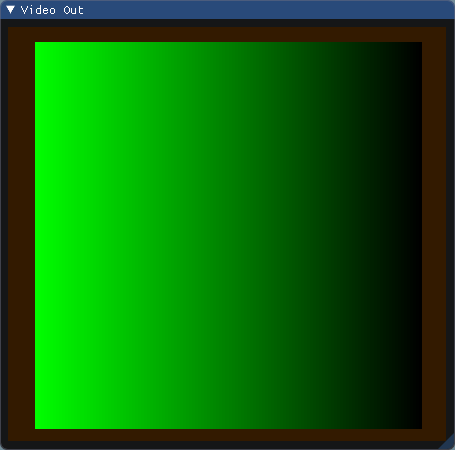
\includegraphics[width=\linewidth]{lab_2_solution}
	\caption{The gradient produced in Lab 2.}
	\label{fig:gradient}
\end{figure}

\subsection{Real-world Interfacing}
The third and final lab asks the student to write a simple program to read input from a button hooked up to a Raspberry Pi and turn on an LED when input is detected. This lab introduces the student to interfacing Cosmic with something physical like a Raspberry Pi. Even though the task in the lab is simple, it opens up a whole new world of opportunities to explore. In Cosmic, Raspberry Pi GPIO pins are mapped to the values in memory from 0xC402 to 0xC41E. The most significant bit in the GPIO bytes signify whether the pin is an input or an output. The remaining 7 bits set it ON or OFF. If the 7 bits equal zero, then the pin if OFF. If they equal something greater than 0, then it is ON. A sample solution is shown in Listing \ref{lab3}.

\begin{lstlisting}[caption={Cosmic assembly to interface with a Raspberry Pi.}, label = {lab3}]
word inputLoc = C402
word outputLoc = C403
start:
	MOV inputLoc R0
    AND FF
	JNZ #turnON
    JMP #turnOFF
turnON:
	MOV FF outputLoc
    JMP #start
turnOFF:
	MOV 80 outputLoc
	JMP #start
\end{lstlisting}

Since the pins are mapped directly to memory in Cosmic, we defined two words to store the input and output locations of the pins we want to use. We then defined a start loop that determines if the LED should be turned on or off based on ANDing the input value with 0xFF and jumping accordingly. If the LED needs to be turned on, the loop jumps to the turnON label that MOVs 0xFF to the output location and jumps back to the start loop. If the LED needs to be turned off, the loops jumps to the turnOFF label that MOVs 0x80 to the output location and jumps back to the start loop. This allows the student to infinitely poll the input from the Raspberry Pi.


\section{Conclusion}
In the end, we could not be happier with the product we delivered. We committed a significant amount of time to Cosmic throughout the last year to get it to where it is now and learned a lot along the way. We hope that Cosmic, or even just the idea of Cosmic, enables and encourages more people to get involved with the retro-computing community and to learn about low level computer design and functionality.


\section{Acknowledgments}
Over the course of this project we posted on multiple relevant forums to get suggestions on how we could improve the system. Through this, many people found our repository and three decided to contribute to the project.

Carsten Eggers (Gwarks) contributed most of the work that went into our graphics system. He holds a lot of knowledge about OpenGL that neither of us did and really helped make that an efficient and useable system.

Akilesh Kannan (aklsh) and Kartik Agaram (akkartik) contributed to making our documentation more accurate.

We'd also like to thank Dr. Li for being our advisor and guiding us through this project. 

\begin{thebibliography}{00}
\bibitem{b0} C. Buxton, K. Carman, "Cosmic". [online] GitHub. Available at: https://github.com/clbx/Cosmic [Accessed 4 May 2020].
\bibitem{b1} Schweighauser, M. (2019). Schweigi/assembler-simulator. [online] GitHub. Available at: https://github.com/Schweigi/assembler-simulator [Accessed 7 Sep. 2019].
\bibitem{b2} GitHub. (2019). Commander X16. [online] Available at: https://github.com/commanderx16 [Accessed 13 Sep. 2019].
\bibitem{b3} "Catch2". [online] GitHub. Available at: https://github.com/catchorg/Catch2 [Accessed 4 May 2020].
\bibitem{b4} "pytest". [online] GitHub. Available at: https://github.com/pytest-dev/pytest [Accessed 4 May 2020].
\bibitem{b5} "Travis CI". [online] Travis CI. Available at: https://travis-ci.org/ [Accessed 4 May 2020].
\end{thebibliography}

\end{document}
